\section{NP-Hardness}
\label{sec:hardness}

In this section, we show that finding the minimum-weight even subgraph in a given homology class is {NP}-hard, even when the underlying surface has no boundary.

Chen and Freedman \cite{cf-qhc-08, cf-qhc2-07} proved a similar hardness result (by reduction from a special case of \textsc{Max2Sat}) for general simplicial complexes; however, the complexes output by their reduction are never manifolds.  Chambers \etal~\cite{ccelw-scsih-08} prove that finding the shortest \emph{splitting} cycle is {NP}-hard; a cycle is splitting if it is non-self-crossing, non-contractible, and null-homologous.  A simple modification of their reduction (from Hamiltonian cycle in planar grid graphs) implies that finding the shortest \emph{strictly simple cycle} in a given homology class is {NP}-hard.  Our proof closely follows a reduction of McCormick \etal~\cite{mrr-edofm-03} from \textsc{Min2Sat} to a special case of \textsc{MaxCut}.

\note{Erin: Feel like we need to cite the totally unimodular Z-homology stuff at some point here too...}

\begin{theorem}
Computing the minimum-cost even subgraph in a given homology class on a surface without boundary is equivalent to computing a minimum-weight cut in an embedded edge-weighted graph $G$ whose negative-cost edges are dual to an even subgraph in $G^*$.
\end{theorem}

\begin{proof}
Fix a graph $G$ embedded on a surface $\Sigma$ without boundary, together with a cost function $c\colon E\to \Real$.  For any even subgraph $H$ of $G$, let $c(H) = \sum_{e\in H} c(e)$, and let $\textsc{MinHom}(H,c)$ denote the even subgraph of minimum cost in the homology class of $H$.

Consider the \emph{residual cost} function $c_H\colon E\to \Real$ defined by setting $c_H(e) = c(e)$ for each edge $e\not\in H$, and $c_H(e) = -c(e)$ for each edge $e\in H$.  For any subgraph $H'$ of $G$, we have $c(H') = c_H(H\oplus H') + c(H)$, which immediately implies that
\(
    \textsc{MinHom}(H,c) ~=~
    H \oplus \textsc{MinHom}(\varnothing, c_H).
\)

Every null-homologous even subgraph of $G$ is dual to a cut in the dual graph $G^*$.  Thus, we have reduced our problem to computing the minimum cut in $G^*$ with respect to the cost function $c_H$.  Since the empty set is a valid cut with zero cost, the cost of the minimum cut is never positive.  In particular, $H$ is the minimum-cost even subgraph in its homology class if and only if the cut in $G^*$ with minimum residual cost is empty.

In fact, our reduction is reversible.  Suppose we want to find the minimum cut in an embedded graph $G = (V, E)$ with respect to the cost function $c\colon E\to \Real$, where every face of $G$ is incident to an even number of edges with negative cost.  Let $H = \set{{e\in E}\mid {c(e)<0}}$ be the subgraph of negative-cost edges, and let $X$ denote the (possibly empty) set of edges in the minimum cut of $G$.  Consider the \emph{absolute cost} function $\abs{c}\colon E^*\to \Real$ defined as $\abs{c}(e^*) = \abs{c(e)}$.  Then $(H\oplus X)^*$ is the even subgraph of $G^*$ of minimum absolute cost that is homologous to $H^*$.
\end{proof}

We now prove that this special case of the minimum cut problem is {NP}-hard, by  reduction from \textsc{MinCut} in graphs with negative edges.  This problem includes \textsc{MaxCut} as a special case (when every edge has negative cost), but many other special cases are also {NP}-hard~\cite{mrr-edofm-03}.  The output of our reduction is a simple triangulation; the reduction can be simplified if graphs with loops and parallel edges are allowed.

Suppose we are given an \emph{arbitrary} graph $G = (V,E)$ with $n$ vertices and an \emph{arbitrary} cost function $c\colon E\to \Real$.  We begin by computing a cellular embedding of $G$ on some surface.  If we don't care whether the surface is orientable, we can simply impose a cyclic order on the edges incident to each vertex.
\note{kylejfox: Won't picking an arbitrary rotation system give us an orientable embedding?}
The maximum-genus \emph{orientable} cellular embedding can be computed in polynomial time~\cite{fgm-fmggi-88}.  Alternately, we can add zero-length edges to make the graph complete and then use classical results of Ringel, Youngs, and others \cite{ry-shmcp-68,r-mct-74} to compute a minimum-genus orientable embedding of $K_n$ in polynomial time.  Once we have an embedding, we add vertices and zero-cost edges to obtain a triangulation.

Let $C$ be the sum of the absolute values of the edge costs: $C:= \sum_e \abs{c(e)}$.  We locally modify both the surface and the embedding to transform each negative-weight edge into a cocycle, as follows.  We transform the edges one at a time; after each iteration, the embedding is a simple triangulation.  (Our reduction can be simplified if a simple graph is not required.)  For each edge~$uv$ with $c(uv)<0$, remove $uv$ to create a quadrilateral face.  Triangulate this face as shown in Figure \ref{F:addhandle}; we call the new faces $uu_1u_2$ and $vv_1v_2$ \emph{endpoint triangles}.  Assign cost $C$ to the edges of the endpoint triangles and cost zero to the other new edges. Glue a new handle to the endpoint triangles, and triangulate the handle with a cycle of six edges, each with cost $c(uv)/6$.  These six edges form a cocycle of cost $c(uv)$, which we call an \emph{edge cocycle}, in the new embedding.  Each iteration adds $5$ vertices and $21$ edges to the graph and increases the genus of the underlying surface by $1$.

\begin{figure}[hbt]
\centering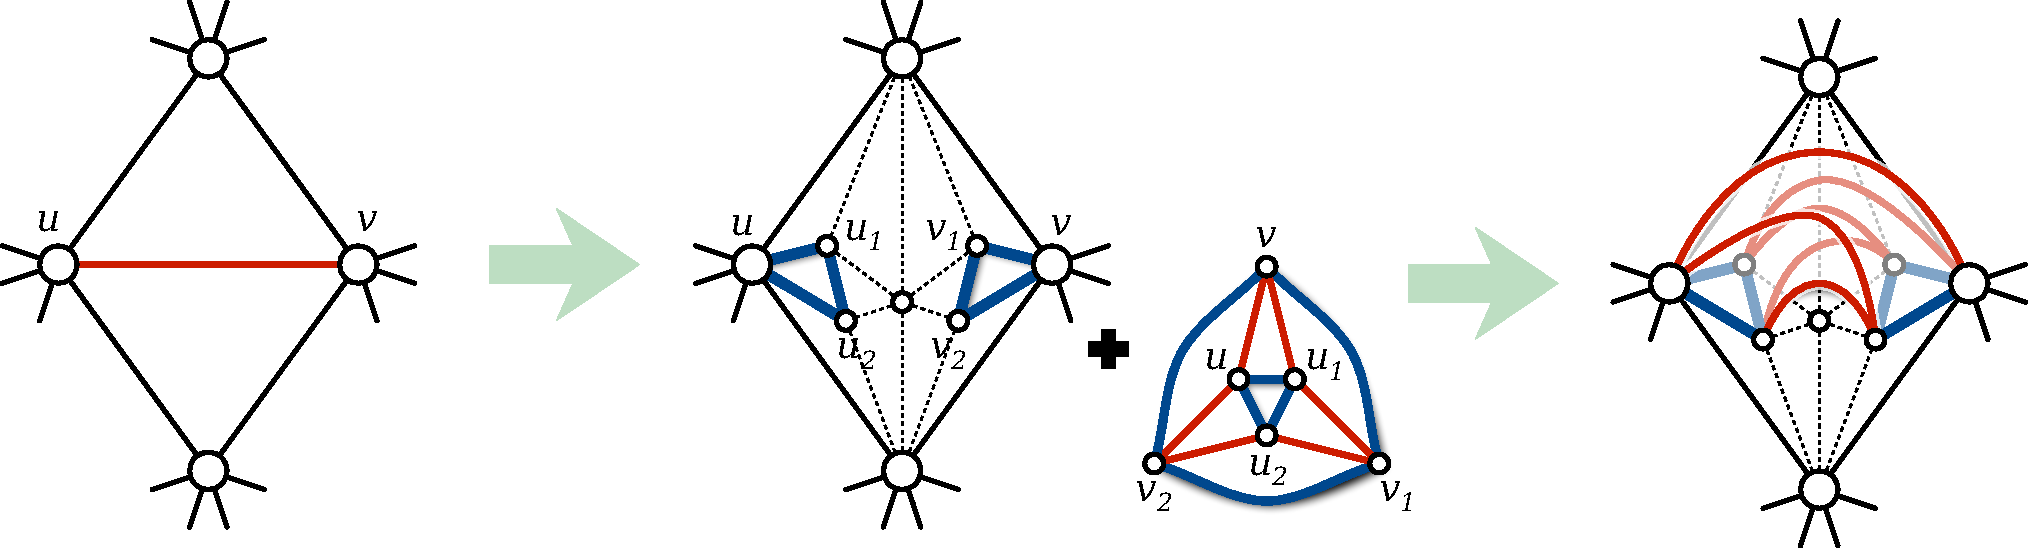
\includegraphics[height=2.25in]{Fig/addhandle3}
\caption{Adding a handle to transform a negative edge into a negative cocycle.  Thick (blue) edges have cost $C$; dashed edges have cost zero.}
\label{F:addhandle}
\end{figure}

Let $G'$ denote the transformed graph and $c'\colon E(G')\to \Real$ its associated cost function.  The minimum cut in $G'$ cannot contain any edge of an endpoint triangle.  Thus, for each edge cocycle, either all six edges cross the cut, or none of them cross the cut.  It follows that the minimum cut in $G'$ corresponds to a cut with equal cost in the original graph $G$.  Conversely, any cut in $G$ can be transformed into a cut in~$G'$ of equal cost.  Thus, computing the minimum cut in $G'$ is equivalent to computing the minimum cut in $G$.

\begin{theorem}
Given an even subgraph $H$ of an edge-weighted graph $G$ embedded on a surface without boundary, computing the minimum-weight even subgraph homologous to $H$ is strongly {NP}-hard.
\end{theorem}

Our reduction can be modified further to impose other desirable properties on the output instances, for example, that the graph is unweighted, every vertex has degree $3$, or the input subgraph $H$ is a simple cycle.
\note{kylejfox: There's a commented out note about how we can further reduce to $3^g$ instances of minimum $(s,t)$-cut in a graph of genus $O(g)$.
Do we want to put that back in?}
%Interestingly, any instance built by our reduction can be further reduced to $3^g$ instances of minimum $(s,t)$-cut in a graph of genus $O(g)$.  For each edge cocycle, we guess which sides of the cut contains its vertex triangles.  If they lie on different sides, we remove the handle, join the vertices on one vertex triangle to a common supersource~$s$, and join the vertices of the other vertex triangle to a common supersink~$t$.  (If they lie on the same side, we do nothing to the cocycle.)  After modifying the graph, we compute the minimum-cost $(s,t)$-cut.

Finally, we emphasize that the {NP}-hardness of this problem relies crucially on the fact that we are using homology with coefficients taken from the finite field $\Z_2$.  The corresponding problem for homology with real or integer coefficients is a minimum-cost circulation problem, and thus can be solved in polynomial time.
Chambers, Erickson and Nayyeri~\cite{cen-hfcc-12} show that this circulation problem can be solved in near-linear time for graphs of constant genus and polynomially bounded integer edge capacities using very different techniques.
\note{Erin: Or cite Hirnani et al unimodular stuff here?}
